\documentclass[11pt]{article}

\usepackage{CMPSC465}
\usepackage{enumitem}
\usepackage{algpseudocode}
\usepackage{tikz}
\usepackage{qtree}

\def\title{Solution 04}

\def\defeq{\mathrel{\mathop:}=}
%\usepackage{algpseudocode}
%\usepackage{algorithm}
\usepackage[ruled,noline]{algorithm2e}
%\usepackage{amsthm}
\newcommand\nonl{%
  \renewcommand{\nl}{\let\nl\oldnl}}% Remove line number for one line
  
\newcommand{\aaa}[1]{\hspace{0.65cm}\parbox[t]{15.3cm}{#1}}
\newcommand{\aab}[1]{\hspace{1.15cm}\parbox[t]{15.0cm}{#1}}
\newcommand{\aac}[1]{\hspace{1.65cm}\parbox[t]{15.0cm}{#1}}
\newcommand{\aad}[1]{\hspace{2.15cm}\parbox[t]{15.0cm}{#1}}
\newcommand{\aaA}[2]{\hspace{0.5cm} {\tikz[overlay] \draw (0.1, -0.1) -- (0.1, #1 * -1.5em + 0.6em);} \parbox[t]{15.0cm}{#2}}
\newcommand{\aaB}[2]{\hspace{1.0cm} {\tikz[overlay] \draw (0.1, -0.1) -- (0.1, #1 * -1.5em + 0.6em);} \parbox[t]{15.0cm}{#2}}
\newcommand{\aaC}[2]{\hspace{1.5cm} {\tikz[overlay] \draw (0.1, -0.1) -- (0.1, #1 * -1.5em + 0.6em);} \parbox[t]{15.0cm}{#2}}
\newcommand{\aaD}[2]{\hspace{2.0cm} {\tikz[overlay] \draw (0.1, -0.1) -- (0.1, #1 * -1.5em + 0.6em);} \parbox[t]{15.0cm}{#2}}
\newcommand{\xxx}{\par\vspace{0.1cm}}

\begin{document}
\maketitle


\begin{qunlist}
\setcounter{sparectr}{-1}
\q{0}{Acknowledgements. }
	The assignment will receive a 0 if this question is not answered.
\begin{enumerate}
	\item If you worked in a group, list the members of the group. Otherwise, write ``I did not work in a group.''
	\item If you received significant ideas about your solutions from anyone not in your group, list their names here. Otherwise, write ``I did not consult  anyone except my group members''.
	\item List any resources besides the course material that you consulted in order to solve the material. If you did not consult anything, write ``I did not consult any non-class materials.''
\end{enumerate}

% 
\q{15}{}
In class, we learned the following property about duality: point $p$ is on line $l$ if and only if point $l^*$ is on line $p^*$.
\begin{enumerate}
    \item Using the property above, prove the following properties:
    \begin{enumerate}
        \item If $n$ points $p_1, ..., p_n$ are on a common line $l$, then $p_1^*, p_2^*, ..., p_n^*$ intersect at a common point $l^*$.
        \item If $n$ lines $l_1, ..., l_n$ intersect at a common point $p$, then $l_1^*, l_2^*, ..., l_n^*$ are on a common line $p^*$.
    \end{enumerate}
    \item If we have a line segment $s$ connecting two points $p_1$ and $p_2$, describe a region $s^*$ corresponding to the dual of $s$ in terms of $p_1^*$ and $p_2^*$. (No rigorous proof is needed.)
    \item If a line $l$ intersects the line segment $s$, prove that $l^*$ is in the region $s^*$.
\end{enumerate}

\textbf{Solution:} 
\begin{enumerate}
    \item
    \begin{enumerate}
        \item For each $p_i$, since $p_i$ is on the line $l$, $l^*$ must be on the line $p_i^*$ in the dual plane. This must hold for every $p_i$, so $l^*$ must be on the lines $p_1^*$, $p_2^*$, ... ,$p_n^*$. Therefore, $p_1^*, p_2^*, ..., p_n^*$ intersect at the common point $l^*$.
        \item For each $l_i$, since $p$ is on the line $l_i$, $l_i^*$ must be on the line $p^*$ in the dual plane. This must hold for every $l_i$, so $l_1^*$, $l_2^*$, ..., $l_n^*$ must be on the line $p^*$. Therefore, $l_1^*, l_2^*, ..., l_n^*$ are on the common line $p^*$.
    \end{enumerate}
    \item The line segment $s$ coincides with a line connecting two points $p_1$ and $p_2$. Let us say this line $l$. Obviously, $p_1^*$ and $p_2^*$ intersects at the point $l^*$ in the dual plain. To figure out the region $s^*$, we investigate where the points on the line segment $s$ will be transformed to the dual plane. For every point $p$ on $s$, $p$ is also on the line $l$. Thus, $p^*$ passes through the point $l^*$. Also, $p$ is in between $p_1$ and $p_2$, so the slope of $p^*$ is in between the ones of $p_1^*$ and $p_2^*$. It means that $p^*$ should be placed in the region between $p_1^*$ and $p_2^*$. This must hold for every $p$ on $s$, hence, $s$ is transformed to the area between $p_1^*$ and $p_2^*$. Without loss of generality, assume $p_1$ is located at the left to the $p_2$, that is, the $x$ coordinate of $p_1$ is less than the one of $p_2$. Then, $s^*$ is the region sweeping from $p_1^*$ to $p_2^*$ in counter-clockwise order. \\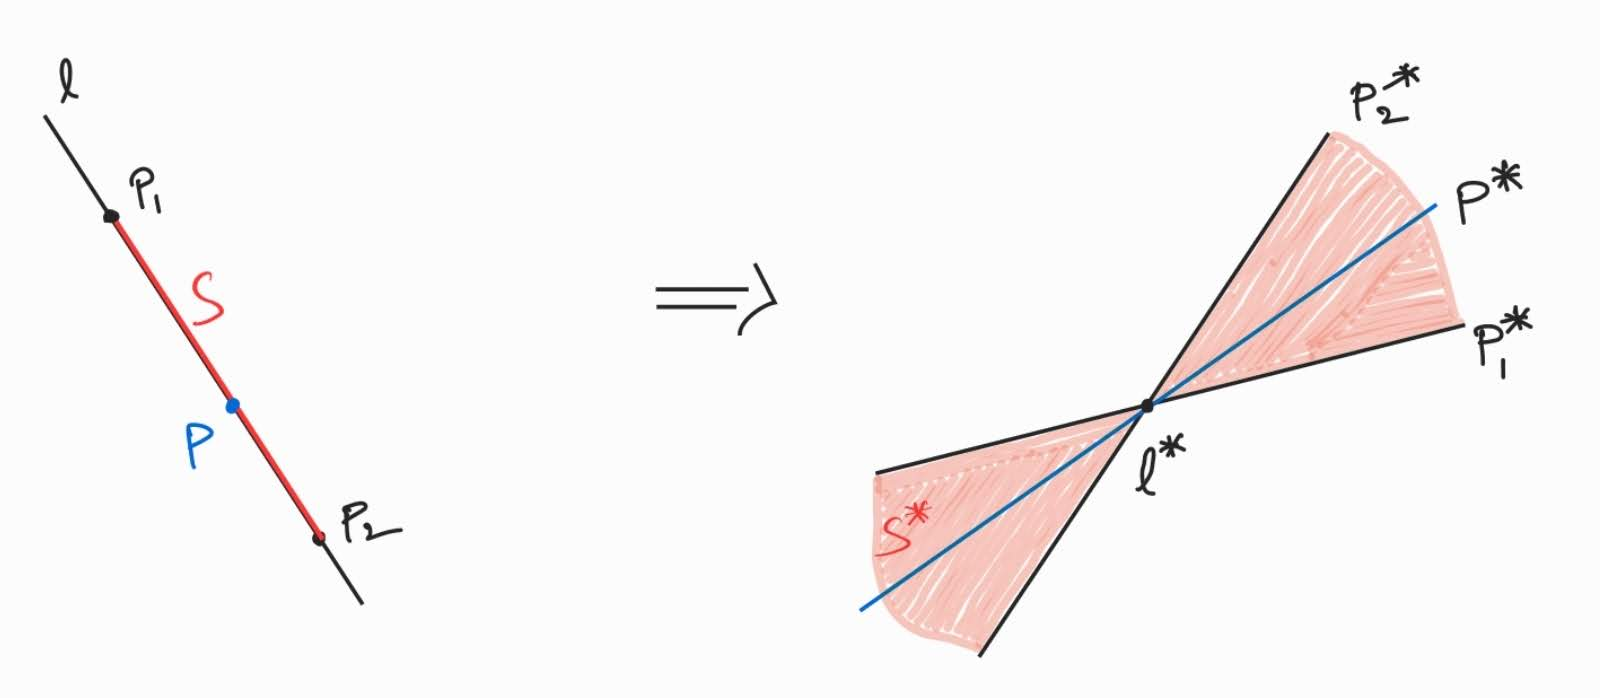
\includegraphics[width=100mm]{region1.jpg}
    \item Since the line $l$ intersects the line segment $s$, there should be a point $p$ on $l$ and $s$. We observe that $p^*$ is in the region $s^*$ from above. Also, we know that $l^*$ is on the line $p^*$, which means $l^*$ is in the region $s^*$.\\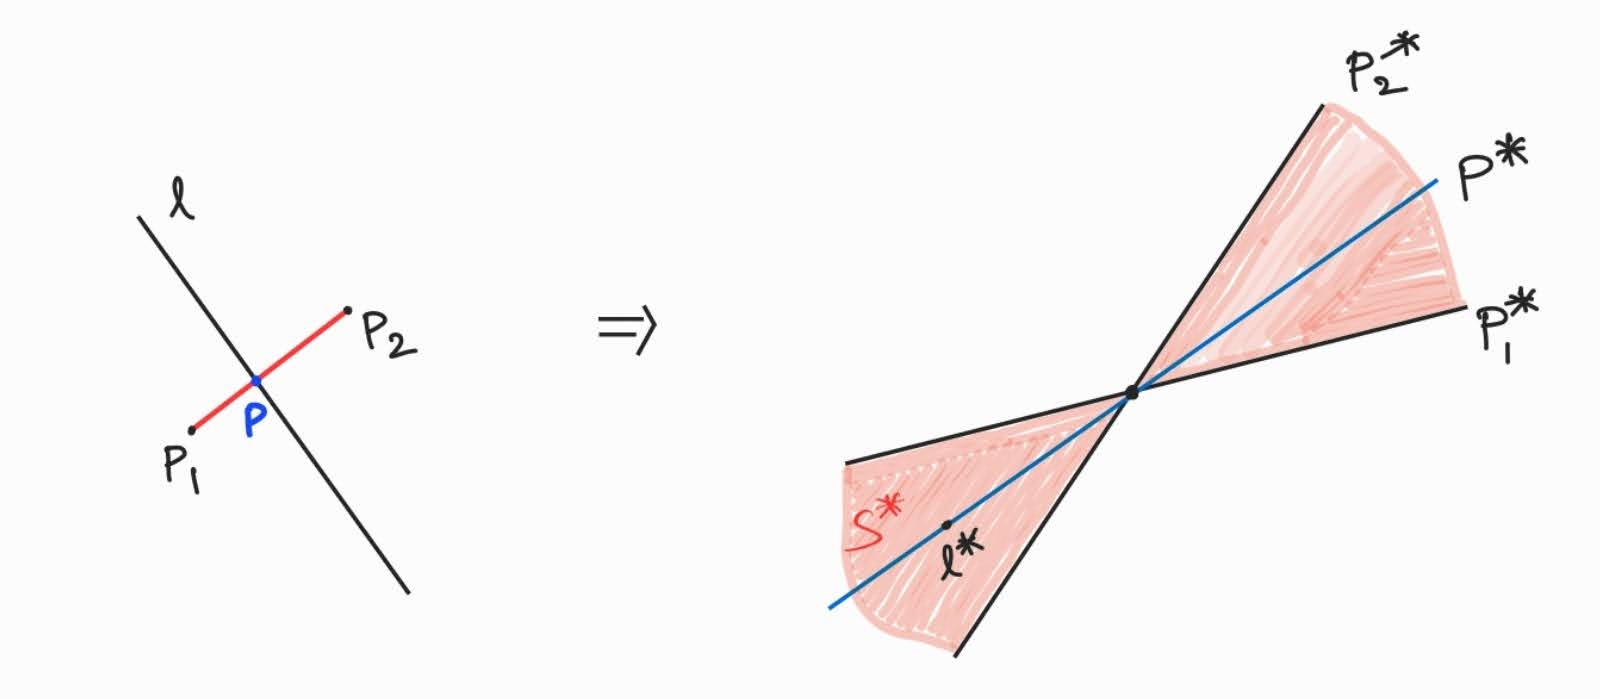
\includegraphics[width=100mm]{region2.jpg}
\end{enumerate}


%Bucky
\q{15}{} We are given a graph $G = (V, E)$; $G$ could be a directed graph or undirected graph. Let $M$ be the adjacency matrix of $G$. Let $n$ be the number of vertices so that the matrix $M$ is $n \times n$ matrix. For any matrix $A$, let us denote the element of $i$-th row and $j$-th column of the matrix $A$ by $A[i, j]$.
\begin{enumerate}
    \item Consider the square of the adjacency matrix $M$. For all $i$ and $j$, show that $M^2[i, j]$ is the number of different paths of length $2$ from the $i$-th vertex to the $j$-th vertex. It should be explained or proved as clearly as possible.\\
    \textbf{Solution:} For any $i$ and $j$, let us find the number of different paths of length 2 from $i$ to $j$. Assume we go through $k$ during our trip. Then, there should be edges between $i$ and $k$ and between $k$ and $j$. In other words, $M[i,k]\cdot M[k,j] = 1$. This path $i \rightarrow k \rightarrow j$ is one of the paths from $i$ and $j$. We need to consider all $k$ for counting the total number of paths, so it should be
    \begin{equation*}
        \sum_{k=1}^n M[i,k] \cdot M[k, j]
    \end{equation*}
    It turns out that it is equal to $M^2[i, j]$.
    
    \item For any positive integer $k$, show that $M^k[i, j]$ is the number of different paths of length $k$  from the $i$-th vertex to the $j$-th vertex. You may use induction on $k$ to prove it.\\
    \textbf{Solution:} We will use induction on $k$.
    \begin{enumerate}
        \item (Base case) $k = 1$ \\ It is clear that $M^k[i,j] = M[i,j]$ has the number of different paths from $i$ to $j$.
        \item (Inductive step) \\ Assume the result is true for $k = l$. It means that $M^l[i, j]$ is the number of different paths of length $l$ from $i$ to $j$. Note that $M^{l+1}[i, j] = \sum_{s=1}^n M^l[i, s] \cdot M[s, j]$ from the matrix multiplication $M^{l+1} = M^l \cdot M$. Every path of length $l + 1$ from $i$ to $j$ consists of paths from $i$ to some vertex $s$ of length $l$ and an edge $s$ to $j$. By the induction hypothesis, $M^l[i, s]$ has the number of different paths of length $l$ from $i$ to $s$. Thus, $M^l[i, s] \cdot M[s, j]$ has the number of different paths of length $l+1$ that is from $i$ to $j$ and located at $s$ at the $l$-th step. Since $s$ is arbitrary, we need to add up over $s$ so $\sum_{s=1}^n M^l[i, s] \cdot M[s, j]$ is the total number of different paths of length $l+1$ from $i$ to $j$.
    \end{enumerate}
    Hence, from $(a)$ and $(b)$, we conclude that $M^k[i,j]$ is the number of different paths of length $k$ from $i$ to $j$ by induction principle.
    
    \item Assume that we are given a positive integer $k$. Design an algorithm to find the number of different paths of length $k$ from the $i$-th vertex to $j$-th vertex for all pairs of $(i,j)$. The time complexity of your algorithm should be $O(n^3 \log k)$. You can get partial credits if you design an algorithm of $O(n^3 k)$.\\
    \textbf{Solution:} Once we have $M^k$ for given $k$, we can get the number of different paths of length $k$ from $i$ to $j$ for any pairs $(i, j)$. It means that we need to design an algorithm to get $M^k$. As the matrix multiplication takes $O(n^3)$, we can come up with a naive algorithm of doing $k-1$ matrix multiplications. In this case, the running time is $O(n^3 k)$. If we reduce the number of matrix multiplications, we will get a better algorithm. \\
    Let $l$ be the highest power of 2 less than or equal to $k$ and $p$ be the exponent of $l$. In other words, $p = \floor{\log_2 k}$ and $l = 2^p$. To do this, let us precompute $M, M^2, M^4, M^8, ..., M^l$. Since $M^{2^i} \cdot M^{2^i} = M^{2^{i+1}}$, we can get $M^2 = M\cdot M$, $M^4 = M^2 \cdot M^2$, $M^8 = M^4 \cdot M^4$, and so on. This precomputation needs $p$ times of matrix multiplication, so it takes $O(n^3 p)$. Next we represent $k$ as a binary number. It has $p + 1$ digits as $2^p \leq k < 2^{p+1}$. \\
    First, we start with the identity matrix $I$. If the first digit is 1, multiply it by $M$. Otherwise, do nothing. After that, if the second digit is 1, multiply it by $M^2$, otherwise, do nothing. If the third digit is 1, multiply it by $M^4$. Repeat this process for $p+1$ digits. With this algorithm, we obtain $M^k$ with at most $p + 1$ times of matrix multiplications. It also takes $O(n^3 p)$. Therefore, our algorithm takes $O(n^3 p)=O(n^3 \log k)$ to get $M^k$ for given $k$.\\
    Example: Let $k = 26$. Then, $l$ is the highest power of 2 less than or equal to $k$, so it is 16, and $p = 4$. Precompute $M, M^2, M^4, M^8$ and $M^{16}$. If we represent $k$ as a binary number, it is $11010_{(2)}$. This implies that $26 = 2^4 + 2^3 + 2^1$. Therefore, $M^{26} = M^{16} \cdot M^8 \cdot M^2$.
\end{enumerate}

% P3
\q{10}{}
You are given a grid of size $n\times m$ and within that grid there is a
horizontal rod~(arbitrary width but height of 1). You aim is to locate it. The only thing you can use to find the
location of the rod is make queries of the form IsPresent~$(x_1,y_1,x_2,y_2)$
where $x_1 \leq x_2 , y_1 \leq y_2$. This returns True if part of the rod is
present in the grid from $(x_1,y_1)$ to $(x_2,y_2)$ and False if not. See figures below.  Design
an algorithm which uses queries $O(\log(n + m))$ times to find the location of the rod, i.e., the leftmost coordinates and rightmost coordinates.
\emph{Hint: consider using binary search in your algorithm.}

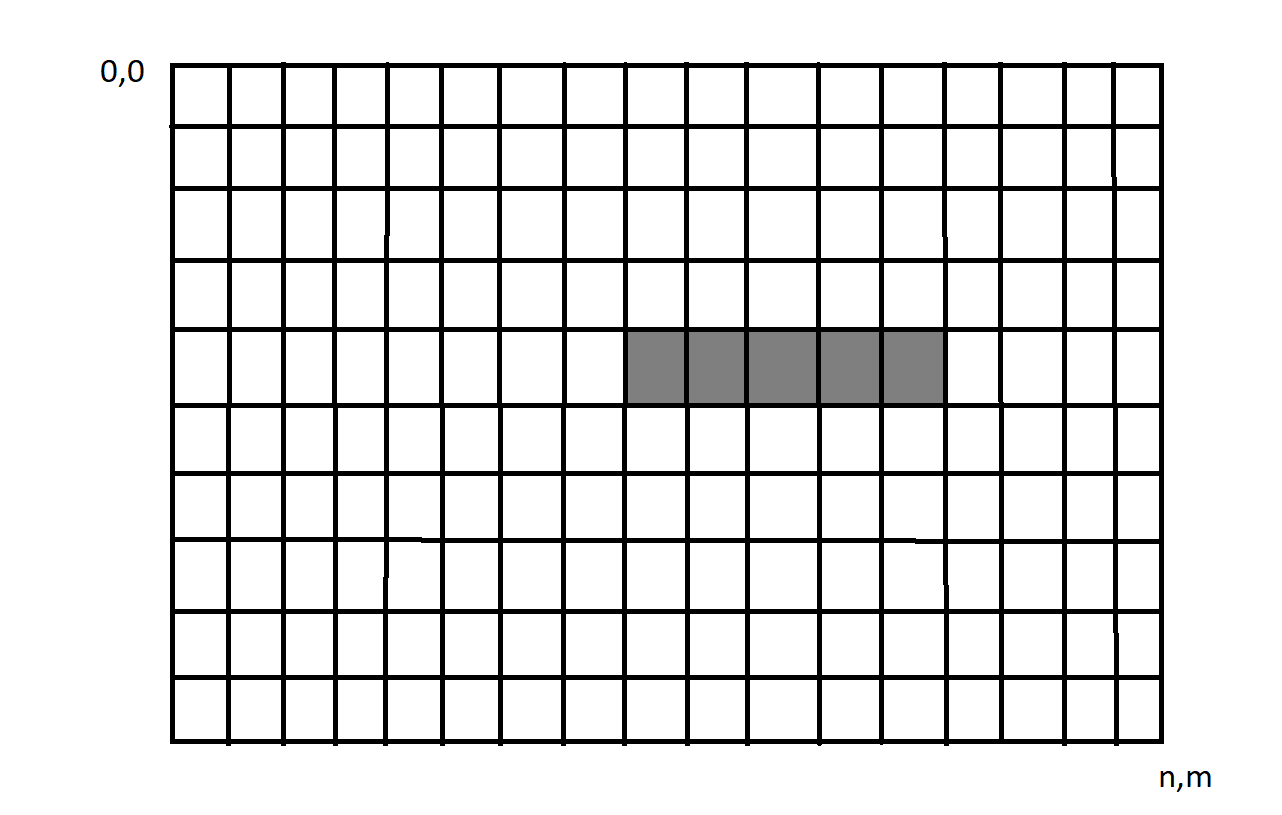
\includegraphics[width=\textwidth]{rod.png}
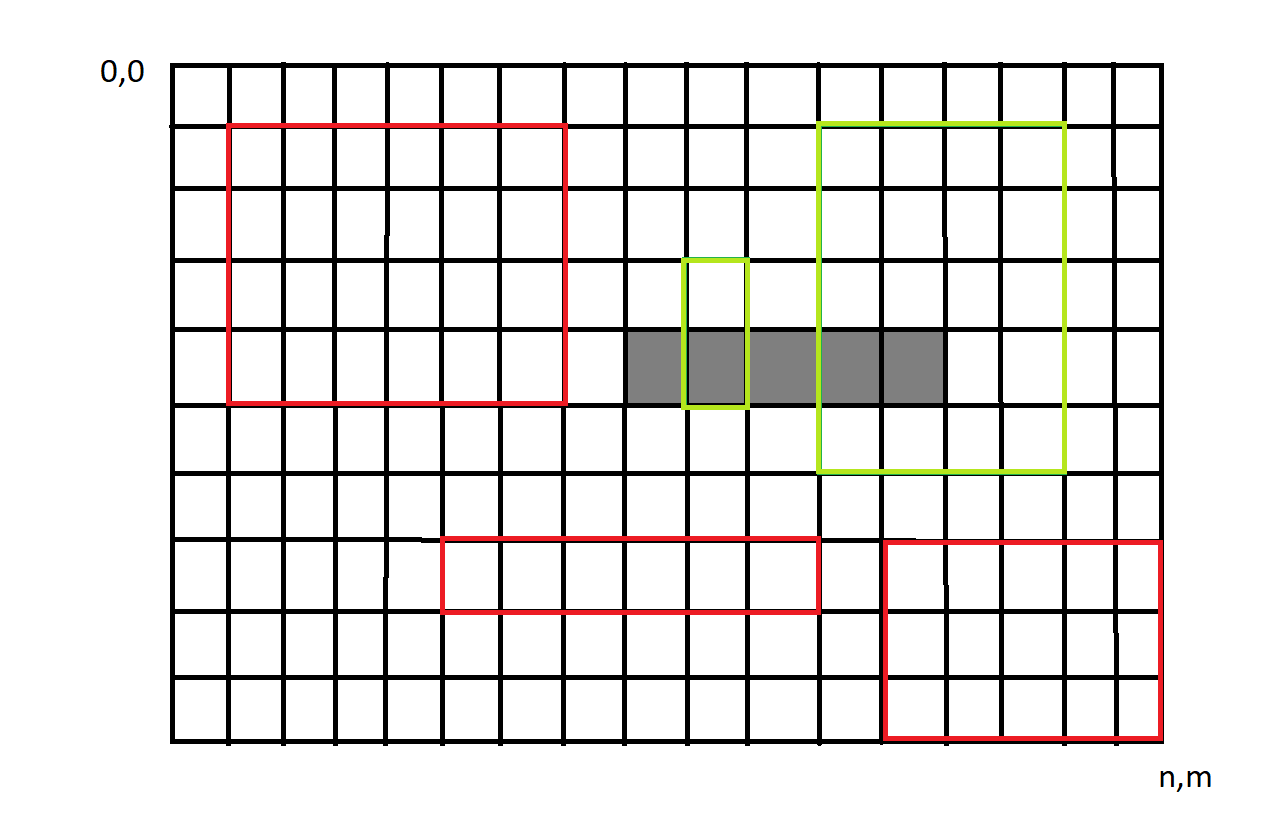
\includegraphics[width=\textwidth]{query.png}

\textbf{Solution:}
\begin{enumerate}
    \item We try to find at which row the rod is located. When making queries, we fix $x_1$ as $0$ and $x_2$ as $n$. Then, we find the upper coordinate and the lower coordinate of the rod by varying $y_1$ and $y_2$ in the same manner as binary search. This step makes $O(\log m)$ queries.
    \item We fix $y_1$ and $y_2$ in any queries later since we found the upper and lower coordinates of the rod. Then, we make queries to find the left coordinate of the rod by varying $x_1$ and $x_2$ in a binary search fashion as well. More specifically, if the current query returns True, we make another query IsPresent~$(x_1,y_1,\floor{\frac{x_2}{2}},y_2)$. On the other hand, if the current query returns False, we make another query IsPresent~$(\floor{\frac{x_1}{2}},y_1,x_2,y_2)$. When $x_2 - x_1 = 1$, we find the leftmost block in the rod, and the leftmost coordinate is $x_1$. This step makes $O(\log n)$ queries.
    \item We find the rightmost coordinate of the rod in a very similar way as step 2. Now, if the current query returns True, we make another query IsPresent~$(\floor{\frac{x_1}{2}},y_1,x_2,y_2)$. If the current query returns False, we make another query IsPresent~$(x_1,y_1,\floor{\frac{x_2}{2}},y_2)$. In the end where $x_2 - x_1 = 1$, we find the rightmost block instead, and the rightmost coordinate is $x_2$. Same as step 2, this step makes $O(\log n)$ queries.
\end{enumerate}
Overall, this algorithm makes $O(\log m) + O(\log n) + O(\log n) = O(\log m + \log n) = O(\log mn)$ queries.\\
Lemma: $O(\log mn) = O(\log (m + n))$\\
Proof:
\begin{itemize}
    \item $m + n \le mn + mn = 2mn$ ($m$ and $n$ can't be positive floats that smaller than 1, based on the semantic of the problem). So, $\log (m + n) = O(\log mn)$.
    \item $mn \le {(m + n)}^2 = m^2 + 2mn + n^2$. So, $\log mn = O(\log (m + n))$.
    \item Consequently, $\log mn = \Theta(\log (m + n))$ and $O(\log mn) = O(\log (m + n))$.
\end{itemize}
From the lemma, our algorithm indeed makes $O(\log mn) = O(\log (m + n))$ queries.

\newpage
{\huge {\bf Rubrics:}}

\bigskip
{\bf Problem 1, 15 pts}
\begin{enumerate}
    \item
    \begin{enumerate}
        \item 3 points : proved/explained 1.a correctly.
        \item 3 points : proved/explained 1.b correctly.
    \end{enumerate}
    \item 5 points : proved/ explained region correctly.
    \item 3 points : partially correct explanation of region.
    \item 4 points : proved that $l^*$ is in the region $s^*$
    \item 2 points : partially correct explanation of $l^*$ is in the region $s^*$.
\end{enumerate}


{\bf Problem 2, 15 pts}
\begin{enumerate}
    \item
    \begin{enumerate}
        \item 3 points : Provided a correct explanation or proof.
    \end{enumerate}
    \item
    \begin{enumerate}
        \item 6 points : Provided a correct proof.
        \item 3 points : Provided an incomplete proof or explanation
    \end{enumerate}
    \item
    \begin{enumerate}
        \item 6 points : Provided an algorithm in $O(n^3 \log k)$
        \item 4 points : Provided an algorithm in $O(n^{\log_2 7} k)$ ($n^{\log_2 7}$ may come from the optimized matrix multiplication in the textbook)
        \item 3 points : Provided an algorithm in $O(n^3 k)$
    \end{enumerate}
    \item 1.5 point : I don't know how to answer this question.
\end{enumerate}

{\bf Problem 3, 10pts}
\begin{itemize}
    \item 3 points: Described a correct way to find at which row the rod is i.e. the uppermost and lowermost coordinates.
    \item 4 points: Described a correct way to find the leftmost and rightmost coordinates.
    \item 3 points: Provided a reasonable running time analysis for the algorithm, and it runs in $O(\log (m + n))$.
    \item 1 point: I don't know how to answer this question.
\end{itemize}


\end{qunlist}
\end{document}
